\chapter{Performance Analysis and Validation}\label{chapter:performance-analysis-validation}

We have thus far discussed the step-by-step implementation of a \ac{FMM}-based solver for the \ac{BEM} formulation of the acoustic scattering problem. In this chapter, we present the results of validating our implementation against analytical solutions, show the effect of using the Burton-Miller formulation, and analyze the performance of our implementation in terms of computational time compared with a traditional \ac{BEM} solver.

\section{Validation vs. Analytical Solution} \label{sec:validation-analytical-solution}
When implementing a new solver, it is critical to validate it against known solutions to ensure it is correctly implemented and produces accurate results. The "acoustic scattering from sound-hard boundaries" problem that we have implemented our solver for has a known analytical solution for a single spherical scatterer in a medium excited by a plane wave.
The plane wave is given by:

\begin{equation*}
    p_{\mathrm{b}}\,=\,p_{0}e^{-i(\mathbf{k}\cdot\mathbf{x})}\,=\,p_{0}e^{-i k_{s}\left({\frac{\mathbf{x}\cdot\mathbf{e}_{k}}{\left|\left|\mathbf{e}_{k}\right|\right|}}\right)}
\end{equation*}
where $p_{0}$ is the amplitude of the plane wave, $\mathbf{k}$ is the wave vector with amplitude $k_s$, $\mathbf{e}_{k}$ is the unit vector in the direction of wave propagation, and $\mathbf{x}$ is the position vector.

The analytical solution for the scattered pressure field is given as a series expansion in terms of spherical harmonics and spherical Bessel functions, as follows:

\begin{equation*}
    p_{s}=p_{0}\left\{\sum_{n=0}^{\infty}\mathrm{i}^{n}(2n+1)\frac{j_{n}^{\prime}(k R)}{h_{n}^{\prime}(k R)}P_{n}(\cos\theta)h_{n}(k r)\right\}
\end{equation*}
where $p_0$ is the amplitude of the incident plane wave, $j_n$ and $h_n$ are the spherical Bessel and Hankel functions of the first kind, respectively, $R$ is the radius of the spherical scatterer, $P_n$ is the Legendre polynomial of degree $n$, $\theta$ is the angle between the direction of wave propagation and the position vector of the external point $\mathbf{x}$ we are computing the scattered field at,  and $r$ is defined as the distance $r = |\mathbf{x}-\mathbf{x}_0|$, with $\mathbf{x}_0$ being the center of the spherical scatterer \cite{marburgburtonmillermethod2016}. 


While the series is infinite, in practice we can truncate it at a finite number of terms, $N$, to obtain an approximation of the scattered field. Our implementation uses a slightly modified version of an empirical formula as shown by \cite{wiscombeimprovedmiescattering1980} to determine the number of terms we use:
\begin{equation*}
    N_{\text{max}} = \left[r ka + 4(ka)^{\frac{1}{3}} + 10 \right]
\end{equation*}
where $ka$ is the size parameter, defined as the product of the wavenumber $k$ and the radius of the scatterer $a$. 

We compare the results of our implementation with the analytical solution using a \texttt{Python} script that computes the analytical solution at all collocation points on the scatterer's surface, and then compares these analytical values with the numerical solution obtained from our \ac{FMM} implementation. 
We run our solver for a single spherical scatterer with the following parameters: 
\begin{itemize}
    \item \textbf{Radius $a$:} 0.1 m
    \item \textbf{Number of elements $N$:} 1533 quad elements
    \item \textbf{Frequency $f$:} 500 Hz
    \item \textbf{Speed of sound $c$:} 343 m/s
    \item \textbf{Wave direction $\mathbf{e}_k$:} [1, 0, 0],  i.e., the wave is propagating in the positive x-direction.
\end{itemize}

This results in a size parameter of $ka =\num{9.159162e-01}$, which gives us $N_{\text{max}} = 14$ using our particular empirical criterion. We find that the results from our implementation match the analytical solution with a relative $L_2$ error, calculated as $ \frac{\| p_{\mathrm{numerical}} - p_{\mathrm{analytical}} \|_2}{\| p_{\mathrm{analytical}} \|_2} $ of $\num{1.062840e-02}$ for the absolute pressure values at the collocation points.
\begin{table}[htbp]
    \centering
    \caption{Error metrics vs. Analytical Solution for scattering from a rigid sphere ($a = 0.1$ m, $f = 500$ Hz, $ka \approx 0.92$).}
    \label{tab:sphere_error_metrics}
    \begin{tabular}{lccc}
        \toprule
        \textbf{Domain} & \textbf{$L_2$ Relative Error} & \textbf{Max Absolute Error ($L_\infty$)} & \textbf{Mean Magnitude Error} \\
        \midrule
        \textbf{Surface} & $1.06 \times 10^{-2}$ (1.06\%) & $2.66 \times 10^{-2}$ & $6.30 \times 10^{-3}$ \\
        \textbf{Slice ($z=0$)} & $5.61 \times 10^{-4}$ (0.05\%) & $7.24 \times 10^{-3}$ & $2.22 \times 10^{-4}$ \\
        \bottomrule
    \end{tabular}
\end{table}

\begin{figure}[htpb]
    \centering
    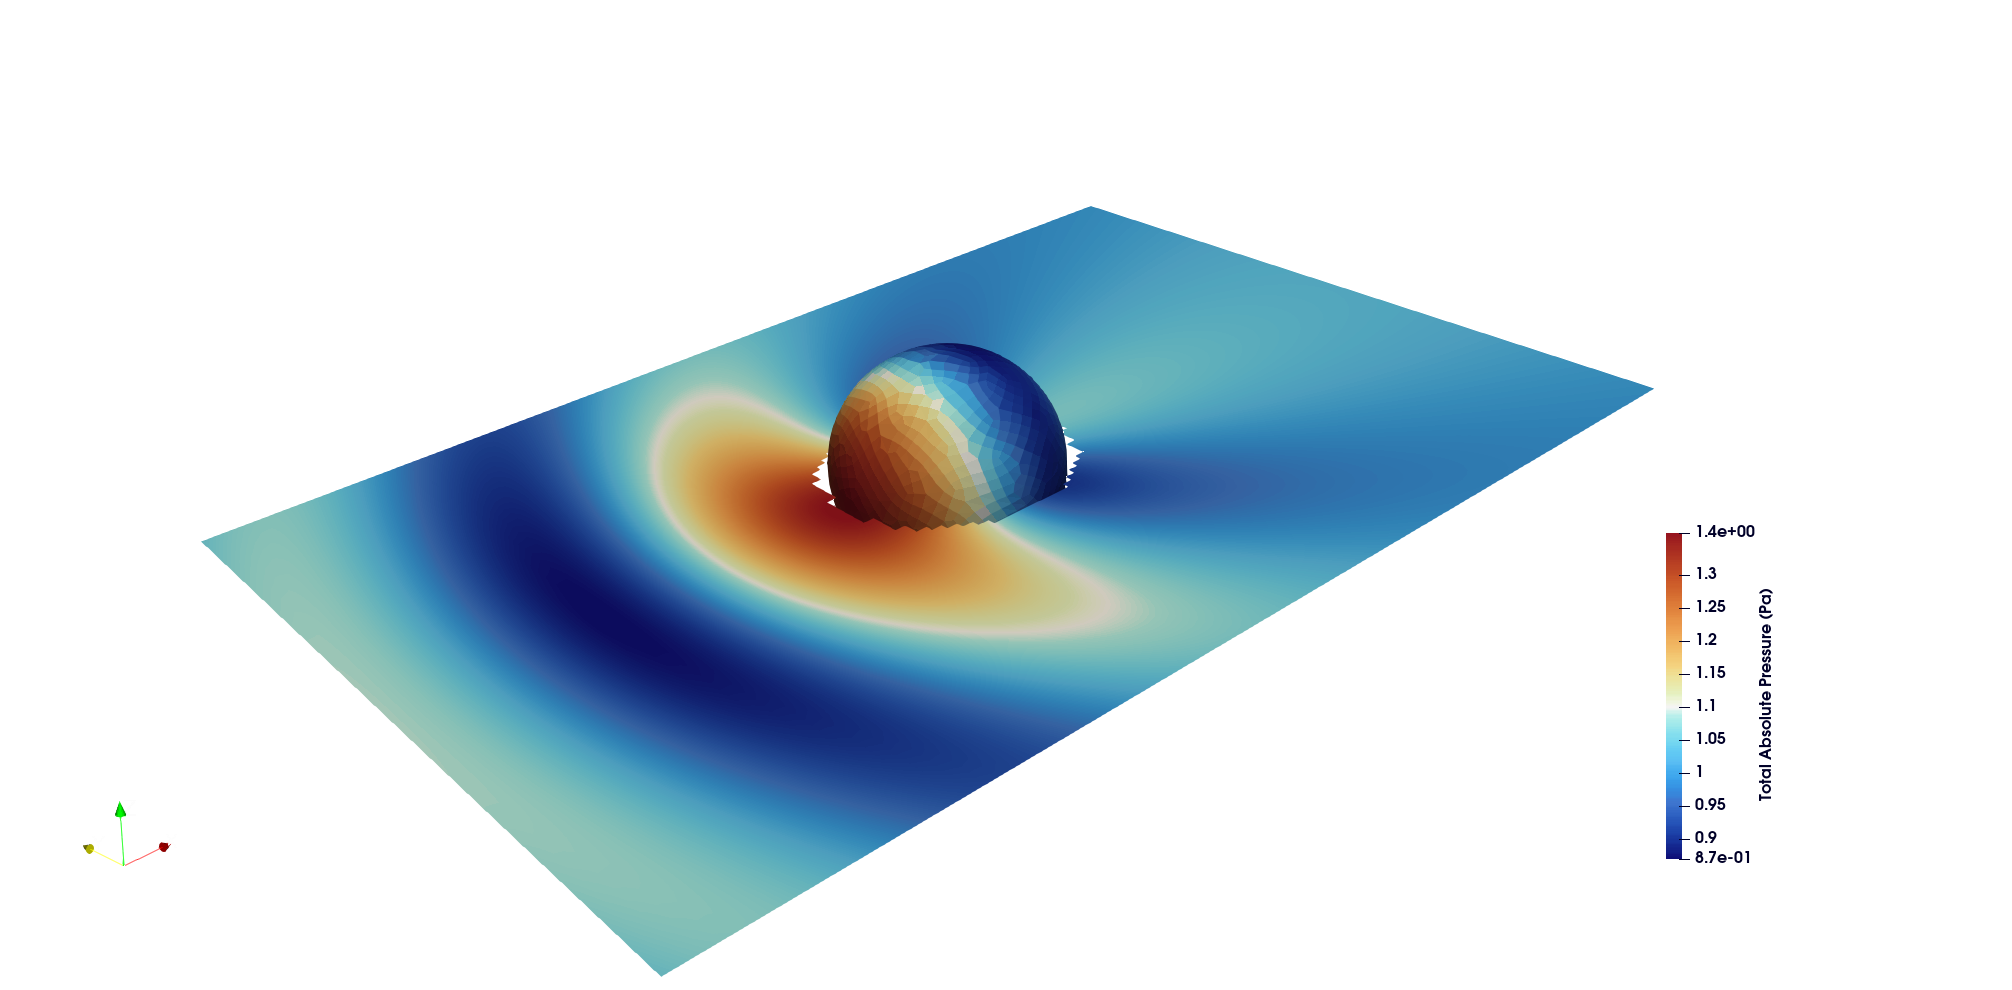
\includegraphics[width=0.8\textwidth]{figures/validation/numerical_absolute_pressure_slice.png}
    \caption{Numerical solution for the total absolute pressure field on a slice on the $z=0$ plane and on the scatterer itself. The spherical scatterer is excited by a plane wave traveling in the positive x-direction, with a frequency of $f = 500$ Hz.}
    \label{fig:sphere_scattering_comparison}
\end{figure}

\begin{figure}[htbp]
    \centering
    
    % --- TOP ROW ---
    % Panel A: Analytical
    \begin{subfigure}[b]{0.49\textwidth}
        \centering
        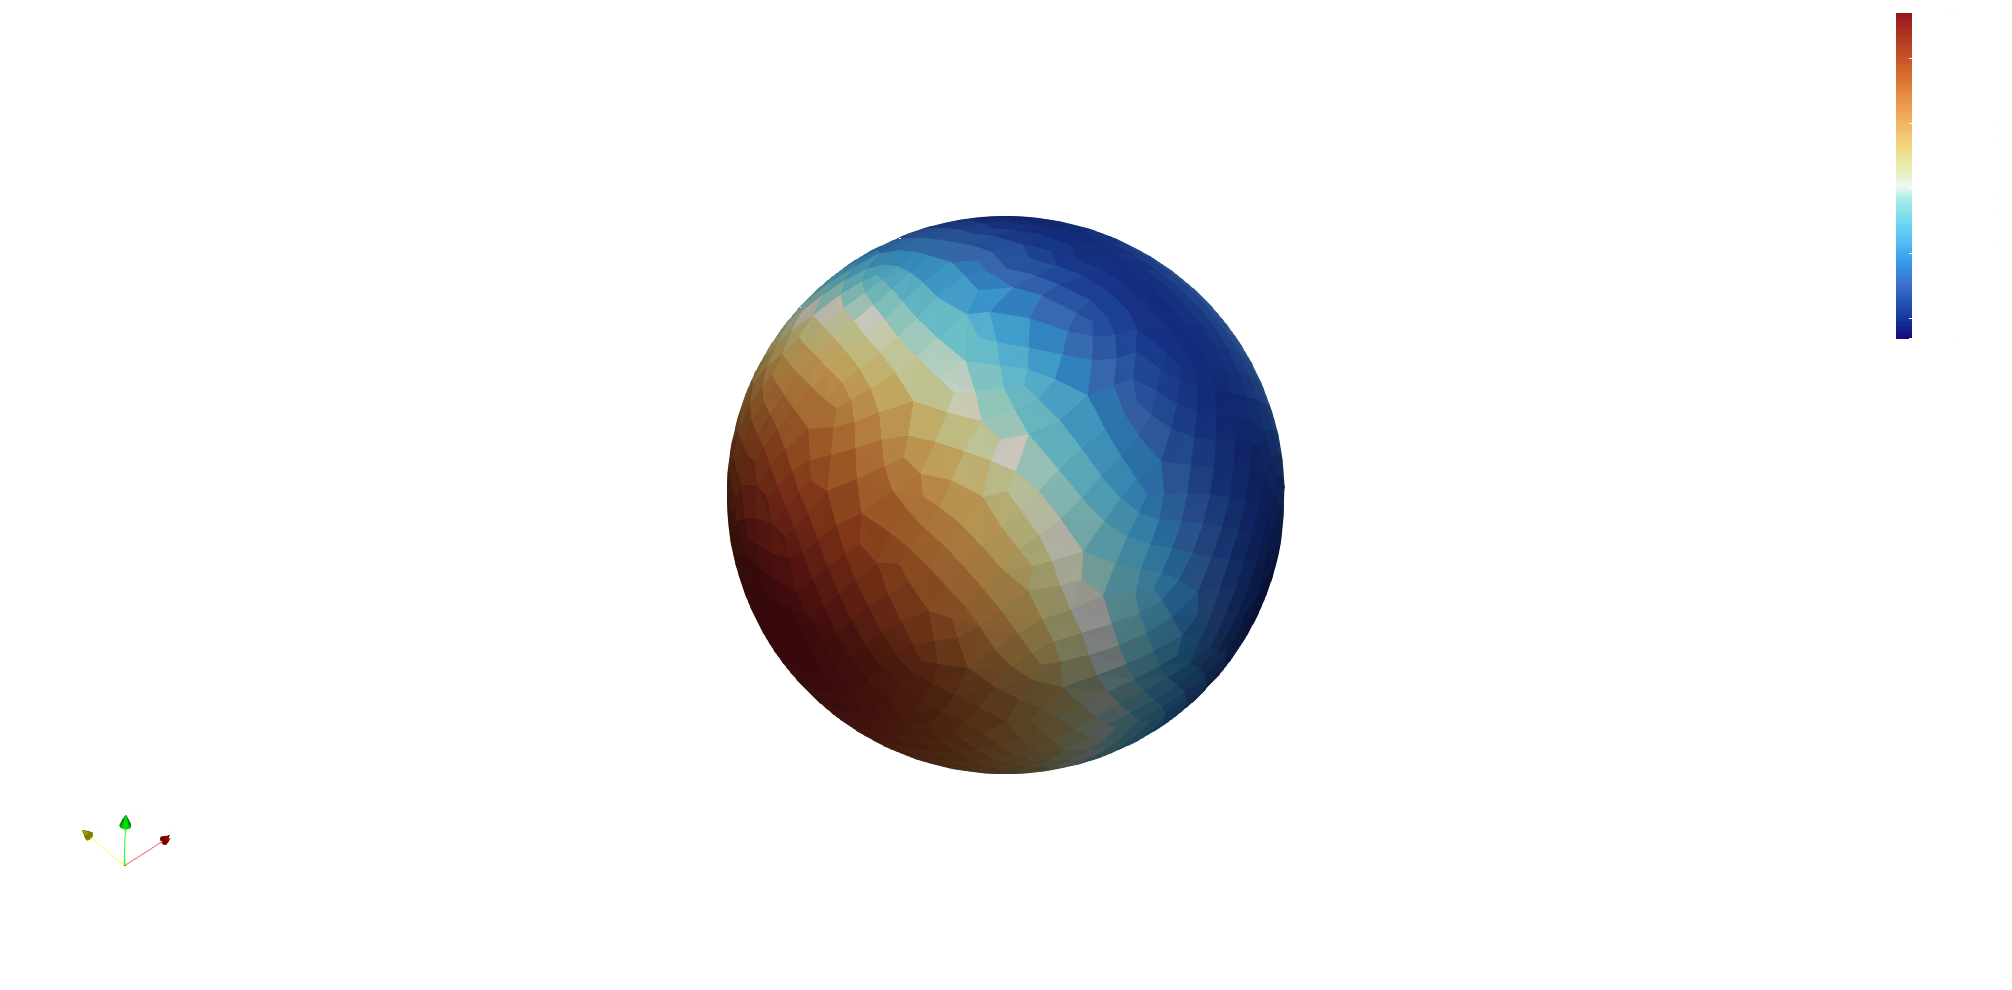
\includegraphics[width=\textwidth]{figures/validation/analytical_absolute_pressure.png}
        \caption{Analytical Solution}
        \label{fig:sphere_ana}
    \end{subfigure}
    \hfill % Pushes the two panels to the margins, creating a 2% gap in the middle
    % Panel B: Numerical
    \begin{subfigure}[b]{0.49\textwidth}
        \centering
        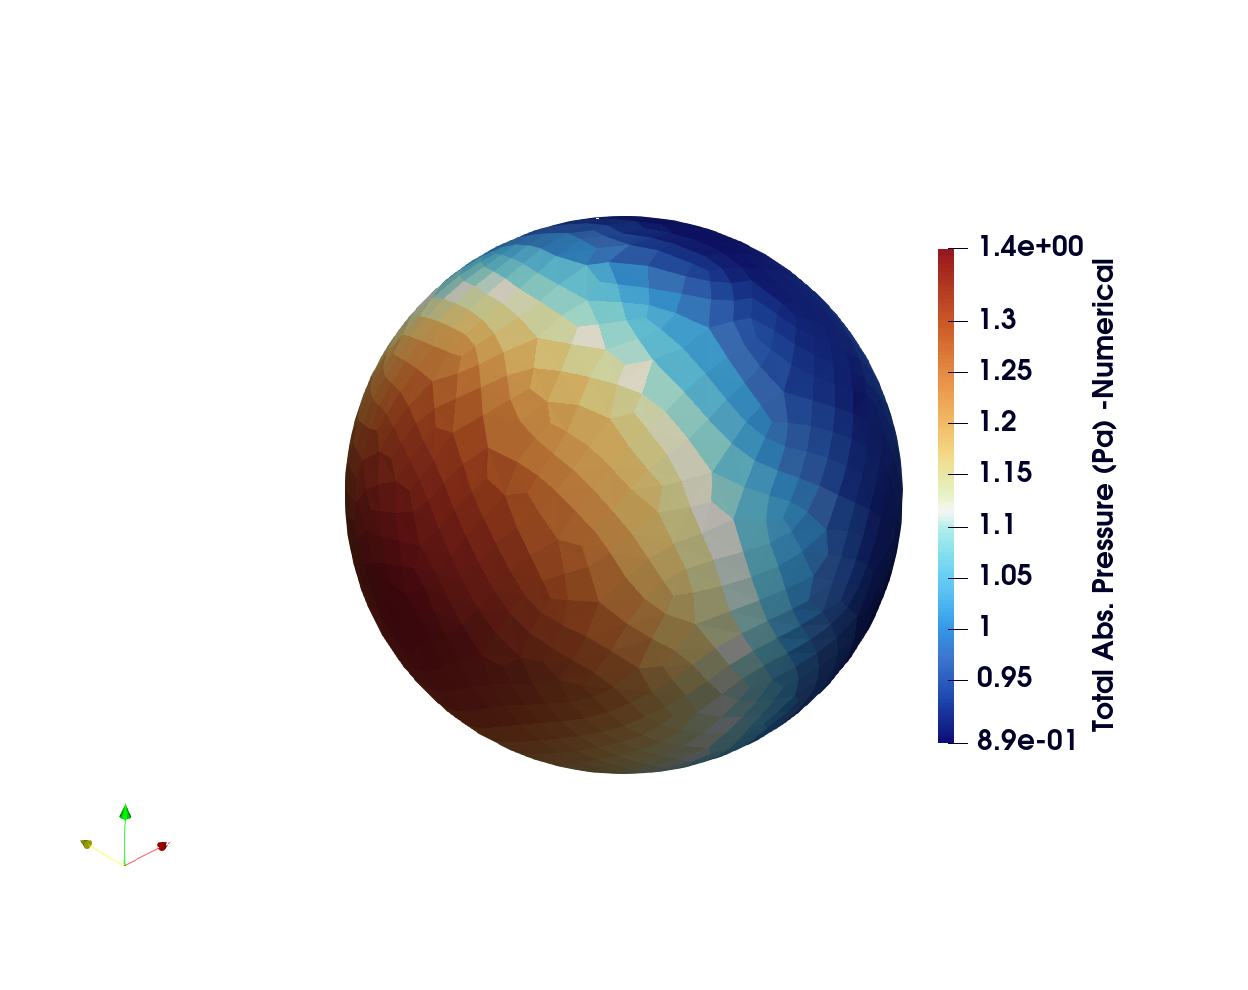
\includegraphics[width=\textwidth]{figures/validation/numerical_absolute_pressure.png}
        \caption{Numerical Solution (BEM)}
        \label{fig:sphere_num}
    \end{subfigure}
    
    \vspace{1em} % Adds a small vertical gap between the top row and the bottom row
    
    % --- BOTTOM ROW ---
    % Panel C: Difference (Centered)
    \begin{subfigure}[b]{0.49\textwidth}
        \centering
        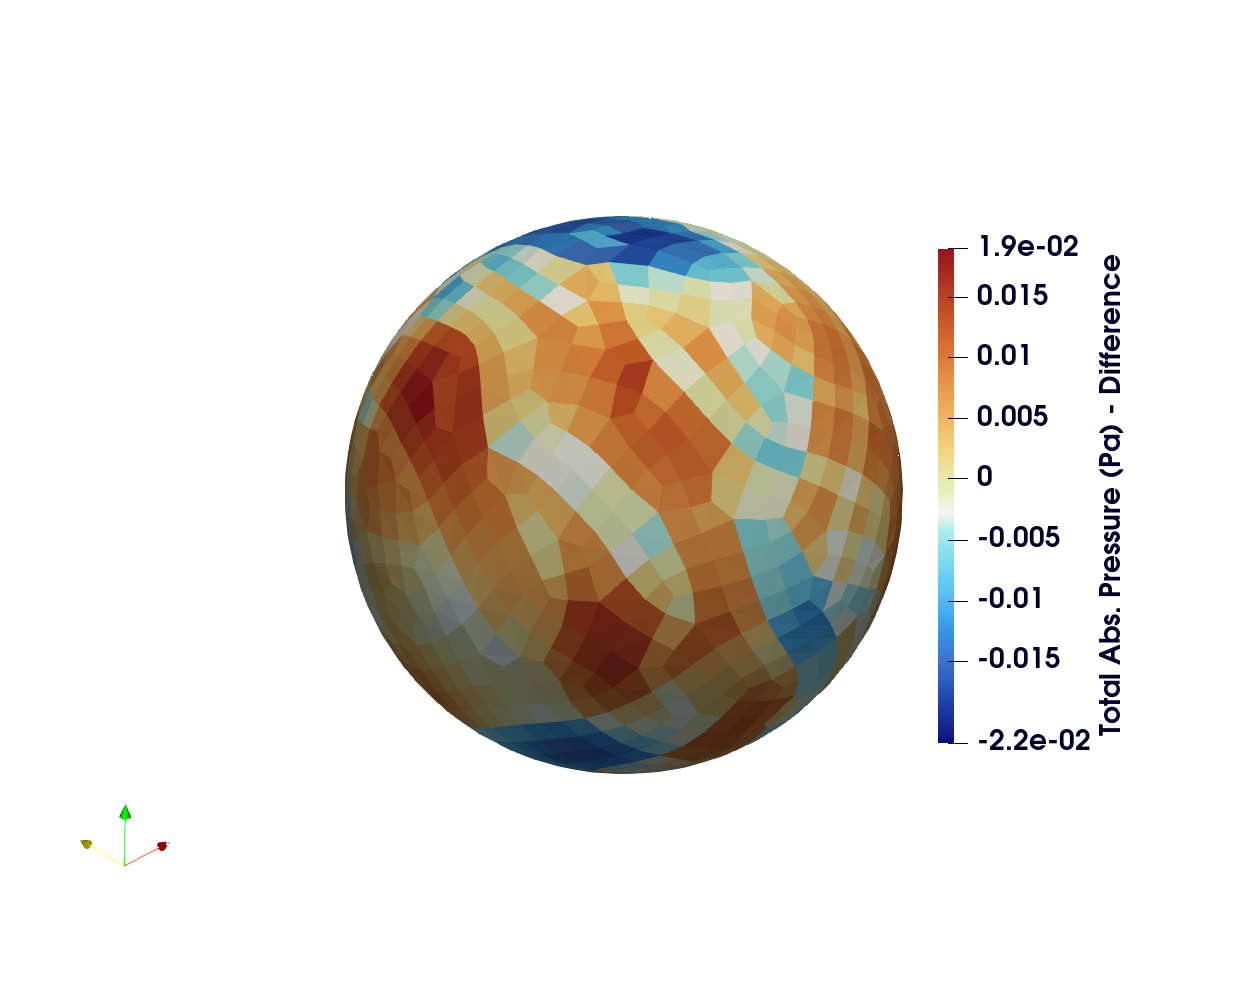
\includegraphics[width=\textwidth]{figures/validation/difference_absolute_pressure.png}
        \caption{Absolute Error Map}
        \label{fig:sphere_diff}
    \end{subfigure}
    
    \caption{Comparison of the surface pressure fields for acoustic scattering by a rigid sphere ($a = 0.1$ m, $f = 500$ Hz, $ka \approx 0.92$). The analytical partial wave series (a) and the \ac{BEM} numerical solution (b) show excellent visual agreement. The absolute error map (c) isolates the local discretization error, which peaks at a magnitude of 0.026.}
    \label{fig:sphere_comparison}
\end{figure}

\section{Effect of the Burton Miller Formulation} \label{sec:effect-burton-miller}
As we have discussed in \autoref{sec:burton-miller}, the \ac{BM} formulation is used to mitigate the non-existence of unique solutions at certain characteristic frequencies. To demonstrate the effect of using the \ac{BM} formulation, we implemented it in our code and toggled it on and off via a command-line flag at runtime. We ran the solver for a sweep of frequencies from $100 Hz$ to $3000 Hz$ for a single spherical scatterer with the same parameters as in \autoref{sec:validation-analytical-solution}, and compared the results with the analytical solution. We especially include the characteristic frequencies, which for a sound-hard sphere are the Dirichlet Resonances, given by the roots of the spherical Bessel function of the first kind, $j_n(ka) = 0$. Our test script has the $ka$ values corresponding to the resonances present within the range of our frequency sweep hardcoded. These fictitious values lying within $100 Hz$ to $3000 Hz$ are:
\begin{enumerate}
\item $f = 1715 Hz$, which corresponds to the first harmonic of a $0.1 m$ radius sphere.
\item $f = 2453 Hz$, which is the first dipole resonance corresponding to a wavenumber $ka =  4.49341$.
\end{enumerate} \cite{klaseboereliminatingfictitiousfrequency2019}. 

\begin{figure}[htpb]
    \centering
    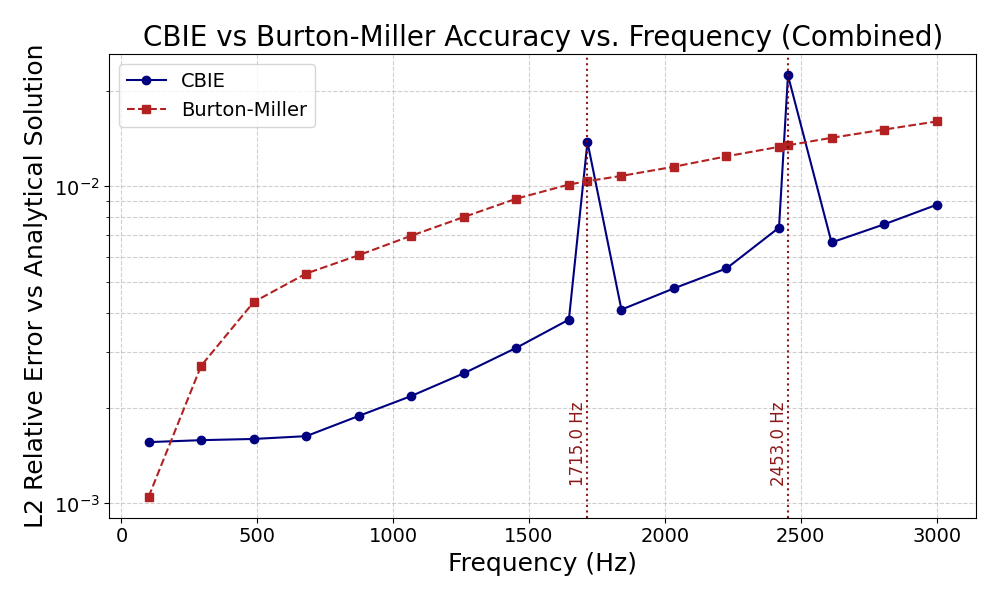
\includegraphics[width=0.8\textwidth]{figures/burton_miller/bem_sweep.png}
    \caption[Frequency sweep Burton-Miller]{Relative $L_2$ error of the numerical solution compared to the analytical solution for a frequency sweep from $100 Hz$ to $3000 Hz$, both with, and without using the \ac{BM} formulation. The spikes is the error of the \ac{CBIE} at the characteristic frequencies (1715 Hz and 2453 Hz) demonstrate the non-uniqueness issue at these frequencies. While the \ac{BM} displays nosuch spikes, its overall error is higher than the \ac{CBIE} formulation, due to the stronger singularity of the \ac{HBIE} kernel compared to the \ac{CBIE} kernel.\ref{sec:effect-burton-miller}}
    \label{fig:frequency_sweep}
\end{figure}

The non \ac{BM} frequency sweep \autoref{fig:frequency_sweep} shows the spikes at the characteristic frequencies, while the one with \ac{BM} \autoref{fig:frequency_sweep} shows that the error at these frequencies is in line with errors at neighboring frequencies, demonstrating the effectiveness of the \ac{BM} formulation in eliminating the non-uniqueness issue at the characteristic frequencies. We can also see that the overall error with the \ac{BM} formulation is slightly higher than without. This is expected, as the \ac{BM} introduces the \ac{HBIE} to the system. As the \ac{HBIE} has a stronger singularity than the \ac{BIE}, the numerical quadrature errors arising from the singularity of the \ac{HBIE} kernel are higher than those arising from the \ac{CBIE} kernel, leading to a higher overall error for the \ac{BM} formulation compared to the non-\ac{BM} formulation.

\section{Performance Analysis} \label{sec:performance-analysis}

The main motivation for implementing the \ac{FMM} is that it offers much better scaling as compared to the traditional \ac{BEM} approach. Traditional \ac{BEM} with direct solvers has a computational complexity of $\mathcal{O}(N^3)$. While the \ac{FMM} has a computational complexity of $\mathcal{O}(N^{\frac{3}{2}})$ or even $\mathcal{O}(N \log N)$ for a multilevel implementation with iterative solvers. This means that even with the additional overhead of managing the hierarchical structure, the \ac{FMM} will break even with, and surpass the performance of the \ac{BEM}. To test the scaling of our \ac{FMM} implementation, we run both the \ac{FMM} and a traditional \ac{BEM} solver on a series of meshes with a grid of identical spherical scatterers, increasing the number of spheres from 1 to 169. We plot the time to set up the system matrix for the traditional \ac{BEM}, compared with the time to set up the \ac{FMM} data structures and precompute the translation operators. We compare the time taken by the direct solver for the traditional \ac{BEM} with the time taken by the GMRES solver for the \ac{FMM}. Lastly, we plot the total time taken by each method as a whole.


\begin{figure}
    \centering
    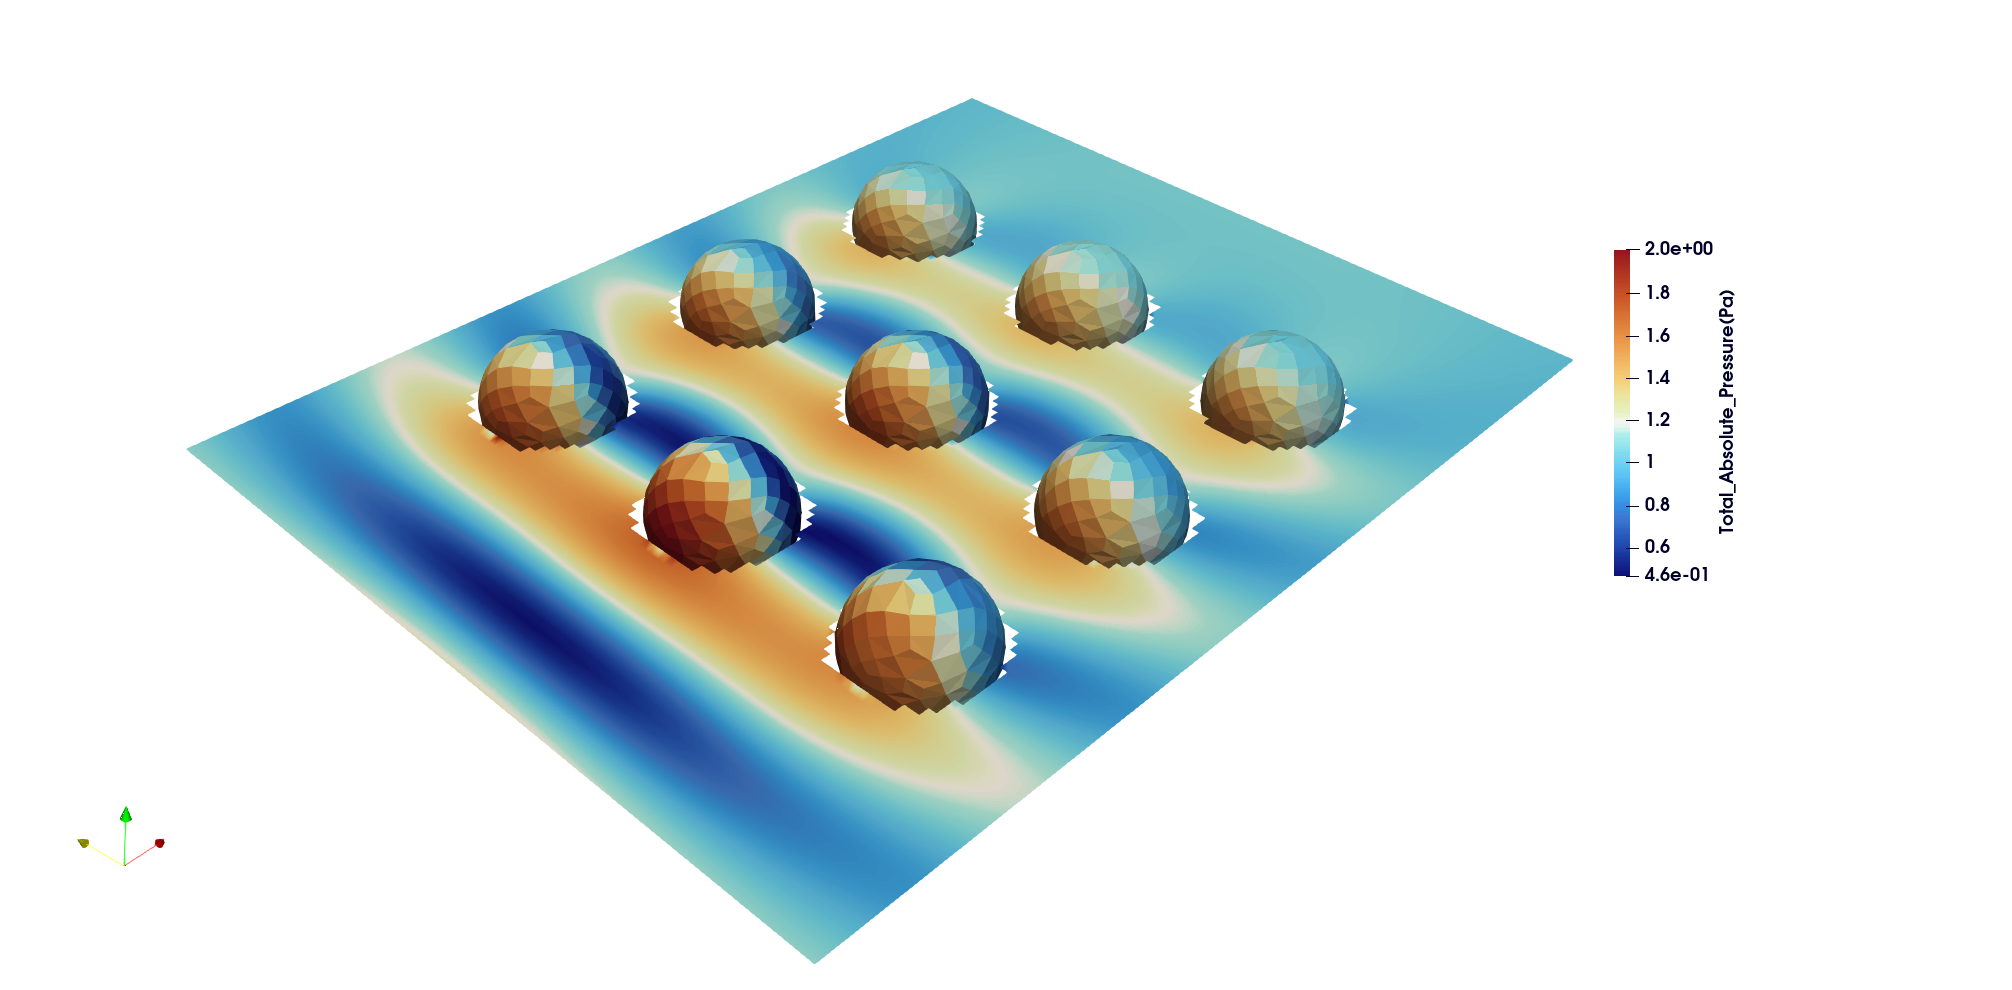
\includegraphics[width=0.8\textwidth]{figures/slice3x3.png}
    \caption[A $3\times 3$ grid of spherical scatterers]{A $3\times 3$ grid of spherical scatterers, in an incident plane wave of frequency $f = 500 Hz$. The plot shows the Total Absolute Pressure (Pa) field on the surface of the scatterers, as well as a slice of the field on the $z=0$ plane.}
    \label{fig:slice3x3}
\end{figure}

\begin{figure}[htpb]
    \centering
    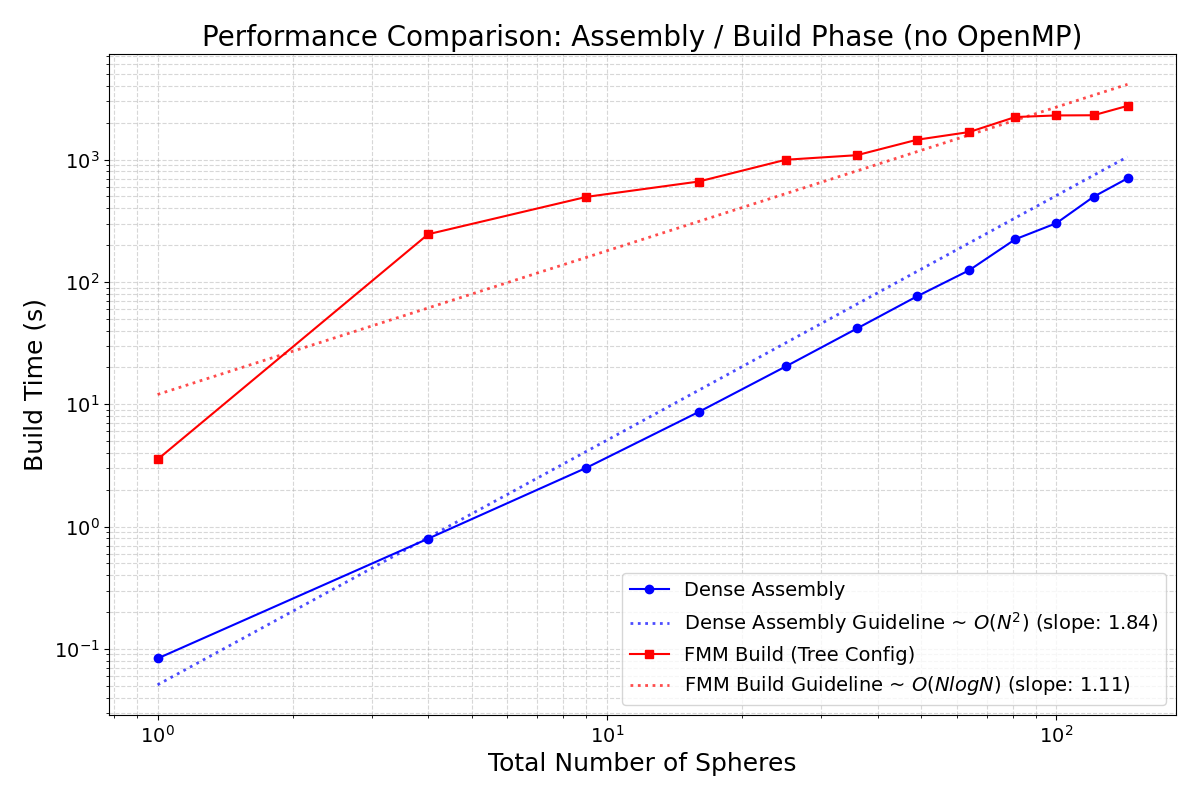
\includegraphics[width=0.8\textwidth]{figures/Timing_Compare_Plots/noOpenMP/timings_comparison_Build_(no_openmp).png}
    \caption[Time to set up the system matrix without OpenMP]{Time taken to set up the system matrix for the traditional \ac{BEM}, as compared to the time taken to set up the \ac{FMM} data structures and precompute the translation operators.}
    \label{fig:setup_time_comparison}
    
\end{figure}

\begin{figure}[htpb]
    \centering
    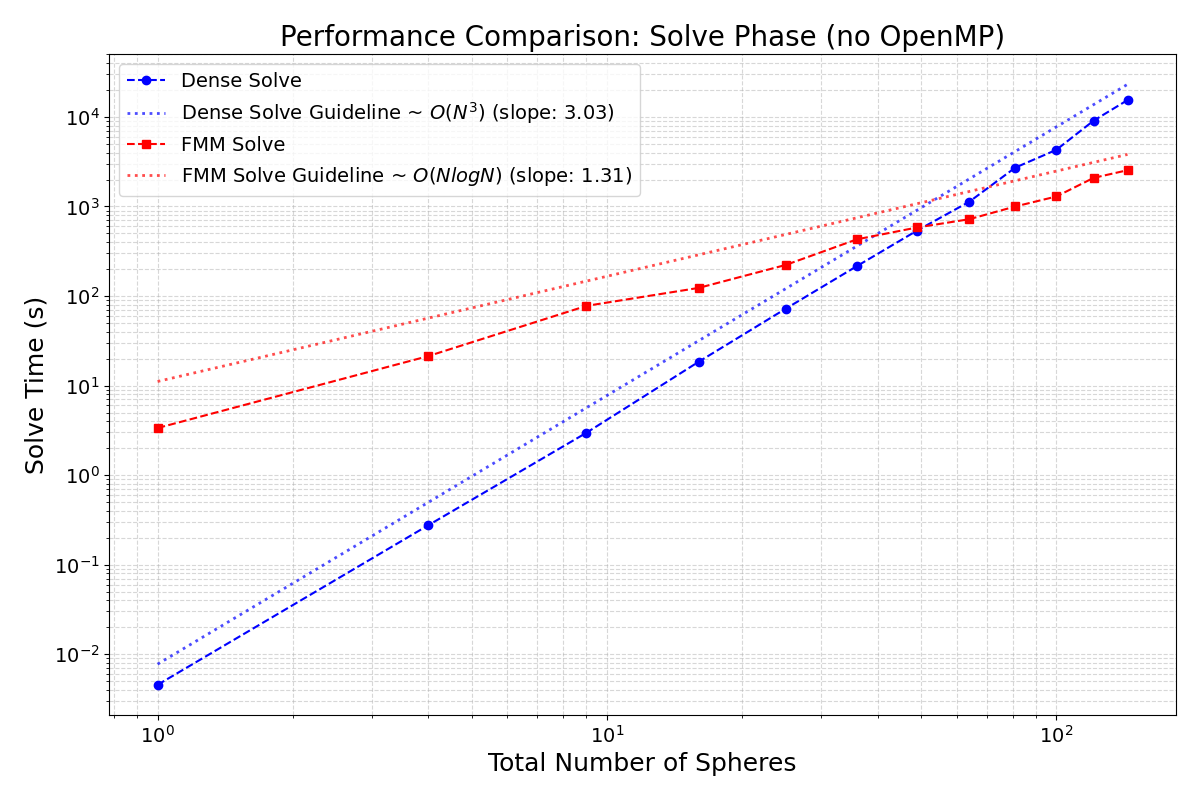
\includegraphics[width=0.8\textwidth]{figures/Timing_Compare_Plots/noOpenMP/timings_comparison_Solve_(no_openmp).png}
    \caption[Time to solve the system without OpenMP]{Time taken to solve the system for the traditional \ac{BEM}, as compared to the time taken to solve the \ac{FMM} system.}
    \label{fig:solve_time_comparison}
    
\end{figure}

\begin{figure}[htpb]
    \centering
    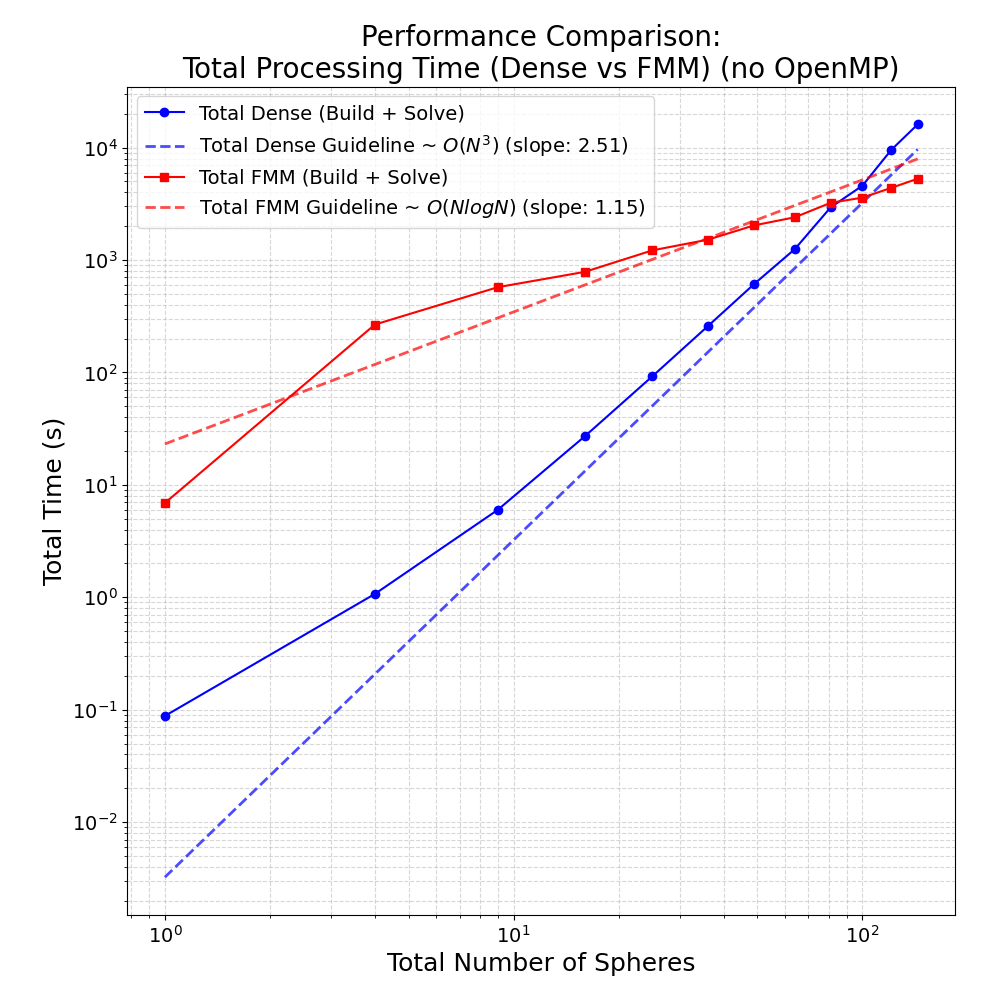
\includegraphics[width=0.8\textwidth]{figures/Timing_Compare_Plots/noOpenMP/timings_comparison_totals_(no_openmp).png}
    \caption[Total time taken without OpenMP]{Total time taken by the traditional \ac{BEM}, as compared to the time taken by the \ac{FMM}.}
    \label{fig:total_time_comparison}
    
\end{figure}



\begin{figure}[htpb]
    \centering
    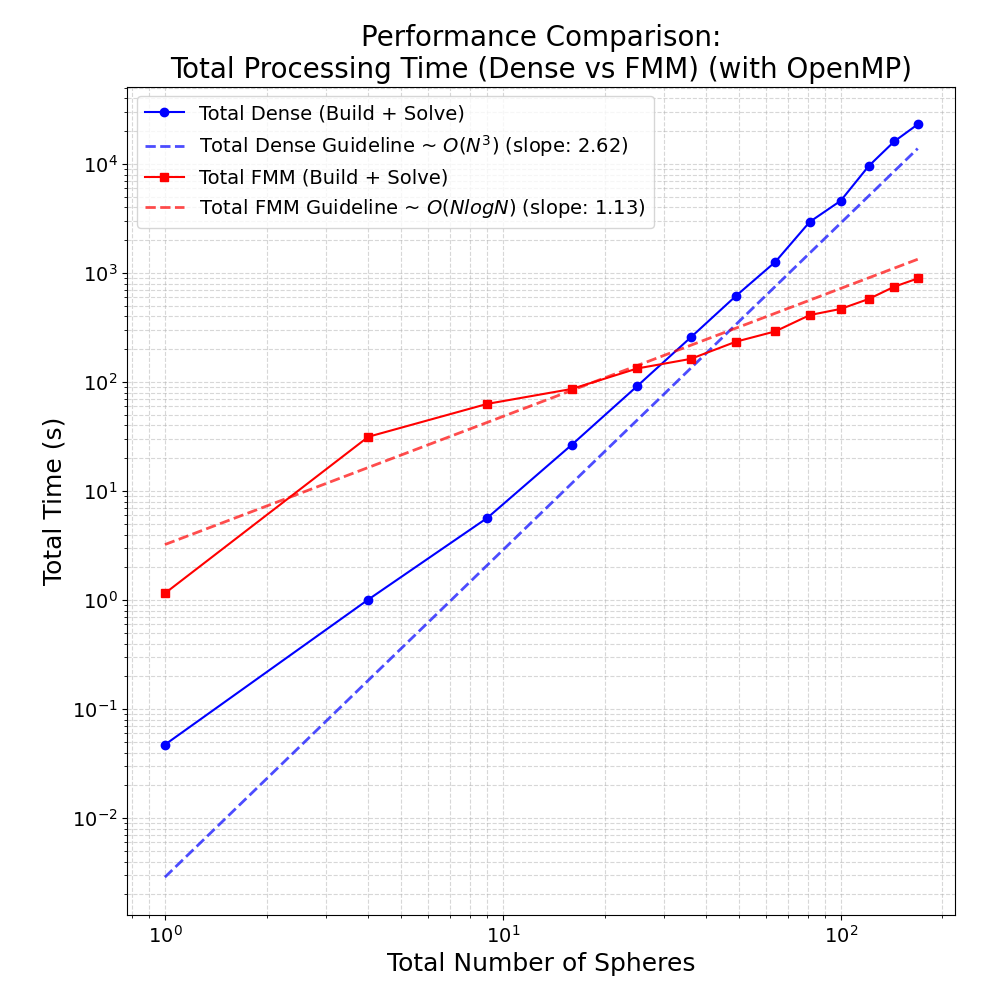
\includegraphics[width=0.8\textwidth]{figures/Timing_Compare_Plots/OpenMP/timings_comparison_totals_(with_openmp).png}
    \caption[Total time taken with OpenMP]{Total time taken by the traditional \ac{BEM}, as compared to the time taken by the \ac{FMM} with OpenMP enabled. The log-log plot enables us to compare the scaling of the two methods. We can see that the \ac{FMM} scales as $\mathcal{O}(N\log N)$, while the traditional \ac{BEM} scales as $\mathcal{O}(N^3)$. The computed slope differs a bit from the theoretical slope, but we can see for the \ac{BEM} it matches the $\mathcal{O}(N^3)$ slope in the asymptote. Meanwhile, the \ac{FMM} may be closer to $\mathcal{O}(N)$ than $\mathcal{O}(N\log N)$}
    \label{fig:total_time_comparison-with_openmp}
\end{figure}

\begin{figure}[htpb]
    \centering
    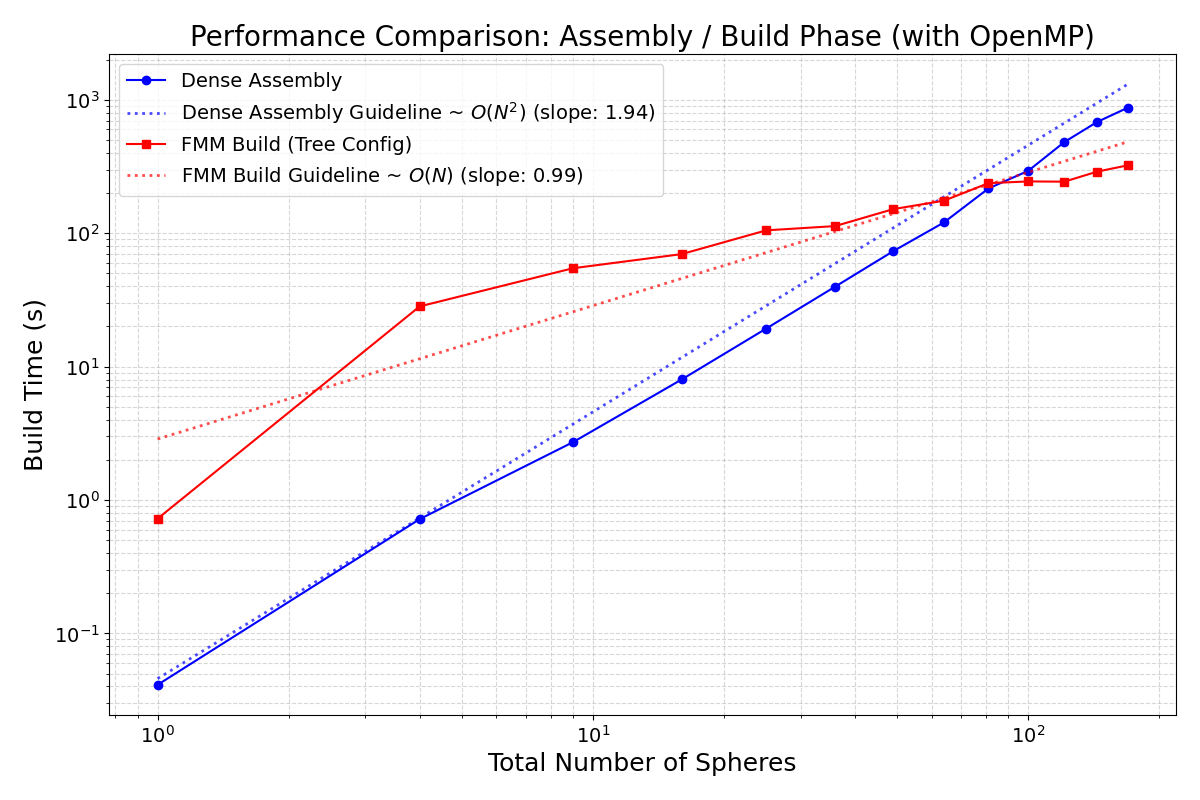
\includegraphics[width=0.8\textwidth]{figures/Timing_Compare_Plots/OpenMP/timings_comparison_Build_(with_openmp).png}
    \caption[Time to set up the system matrix with OpenMP]{Time taken to set up the system matrix for the traditional \ac{BEM}, as compared to the time taken to set up the \ac{FMM} data structures and precompute the translation operators. The Dense \ac{BEM} matrix assembly takes $\mathcal{O}(N^2)$ time, while the \ac{FMM} build time scales as $\mathcal{O}(N)$.}
    \label{fig:setup_time_comparison-with_openmp}
    
\end{figure}

\begin{figure}[htpb]
    \centering
    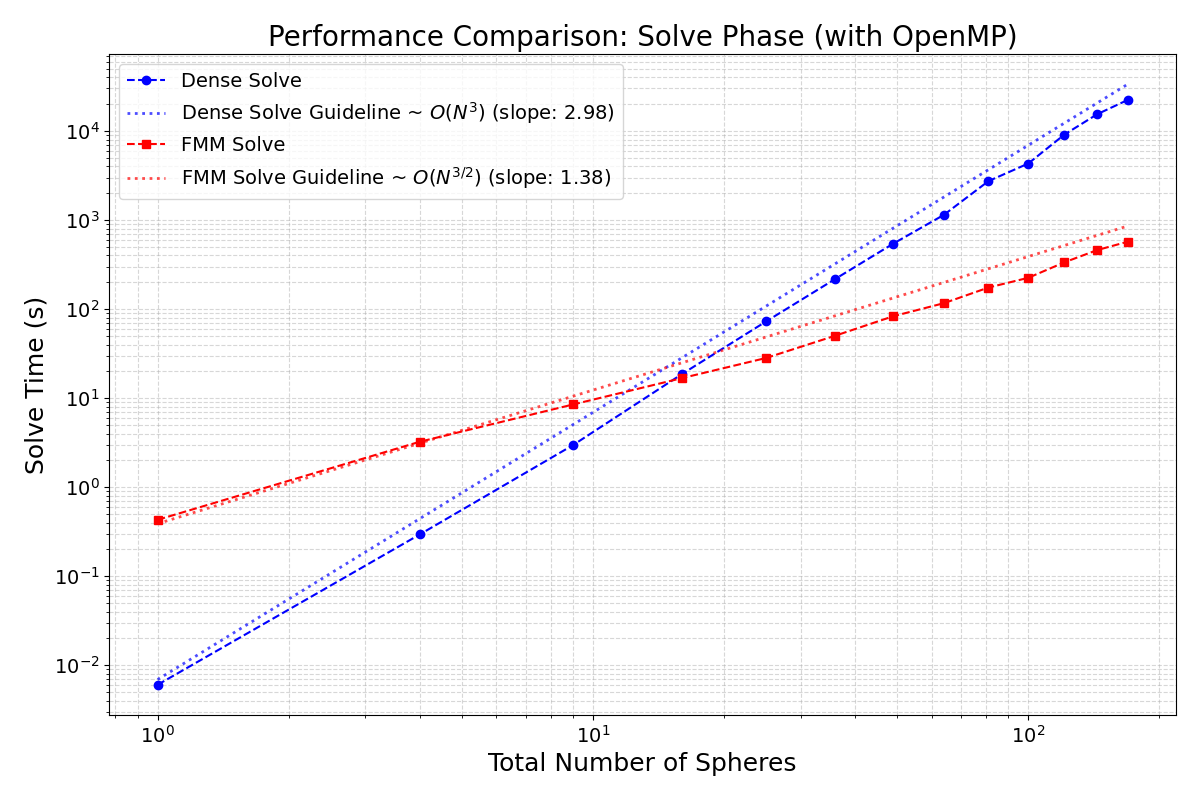
\includegraphics[width=0.8\textwidth]{figures/Timing_Compare_Plots/OpenMP/timings_comparison_Solve_(with_openmp).png}
    \caption[Time to solve the system with OpenMP]{Time taken to solve the system for the traditional \ac{BEM}, as compared to the time taken to solve the \ac{FMM} system. The \ac{FMM} with its iterative \ac{GMRES} coupled with the fast matrix-vector products scales as $\mathcal{O}(N^{\frac{3}{2}})$, while the direct solver for the traditional \ac{BEM} scales as $\mathcal{O}(N^3)$. The Direct \ac{BEM} solver uses matrix inversion to solve the system, which is quite an expennsive operation.}
    \label{fig:solve_time_comparison-with_openmp}
    
\end{figure}


In all these timing plots \autoref{fig:setup_time_comparison-with_openmp}, \autoref{fig:solve_time_comparison-with_openmp}, and \autoref{fig:total_time_comparison-with_openmp}, we have included guidelines corresponding to the closest asymptotic complexity for each timing curve.
Let us consider the traditional \ac{BEM} first. The time taken to set up the system matrix scales as $\mathcal{O}(N^2)$, as we have to compute the interaction between every pair of elements. The time taken to solve the system scales as $\mathcal{O}(N^3)$, but considering the solving time makes up the bulk of the total time needed for the traditional \ac{BEM}, the total time also scales as $\mathcal{O}(N^3)$.
The \ac{FMM} build time scales as $\mathcal{O}(N)$. This time is dominated by the time spent computing the \ac{M2L} translation operators, the number of which scales somewhat linearly with $N$ elements. The solution time taken by the Real-Equivalent system with \ac{GMRES} scales as $\mathcal{O}(N^{\frac{3}{2}})$. As the amount of overhead needed to set up the \ac{FMM} data structures and precompute the translation operators goes down as a percentage of the total time taken as $N$ increases, the total time taken by the \ac{FMM} scales as $\mathcal{O}(N\log N)$\cite{chengwidebandfastmultipole2006}.

The plots \autoref{fig:setup_time_comparison-with_openmp}, \autoref{fig:solve_time_comparison-with_openmp}, and \autoref{fig:total_time_comparison-with_openmp}, were run with OpenMP on a system with 24 Threads. The \ac{BEM} parat of the code does not leverage OpenMP, so we also include plots with OpenMP disbled to show a fair comparison of the scaling of the two methods without the effect of parallelization. The plots with OpenMP disabled are \autoref{fig:setup_time_comparison-no_openmp}, \autoref{fig:solve_time_comparison-no_openmp}, and \autoref{fig:total_time_comparison-no_openmp}. We can see that the \ac{FMM} time complexity remains the same in the single-threaded case, just with higher absolute times. The \ac{BEM} times are unaffected as they did not leverage OpenMP in the first place. Both sets of plots demonstrate that as the problem size increases, the \ac{FMM} sooner or later breaks even with the \ac{BEM} and outperforms it.
\begin{figure}[htpb]
    \centering
    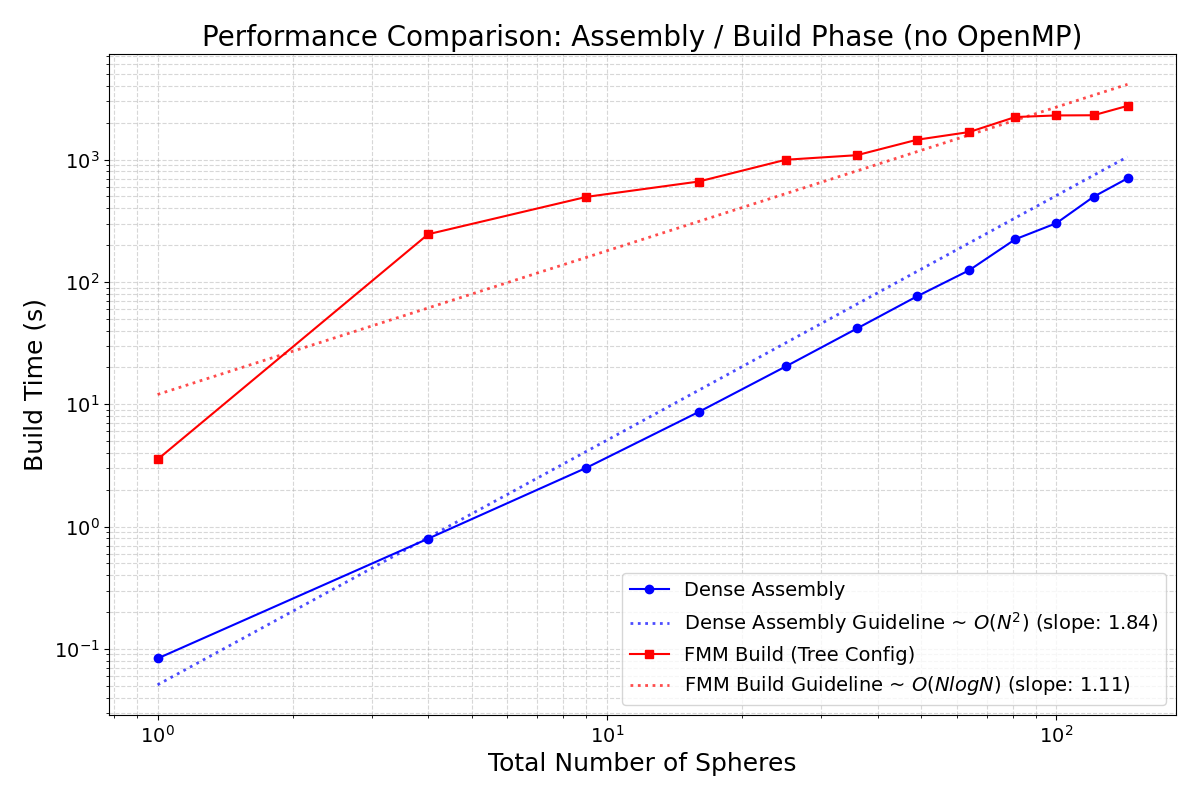
\includegraphics[width=0.8\textwidth]{figures/Timing_Compare_Plots/noOpenMP/timings_comparison_Build_(no_openmp).png}
    \caption[Time to set up the system matrix without OpenMP]{Time taken to set up the system matrix for the traditional \ac{BEM}, as compared to the time taken to set up the \ac{FMM} data structures and precompute the translation operators. The Dense \ac{BEM} assembly takes $\mathcal{O}(N^2)$ time, while the \ac{FMM} build time scales as $\mathcal{O}(N)$.}
    \label{fig:setup_time_comparison-no_openmp}
    
\end{figure}

\begin{figure}[htpb]
    \centering
    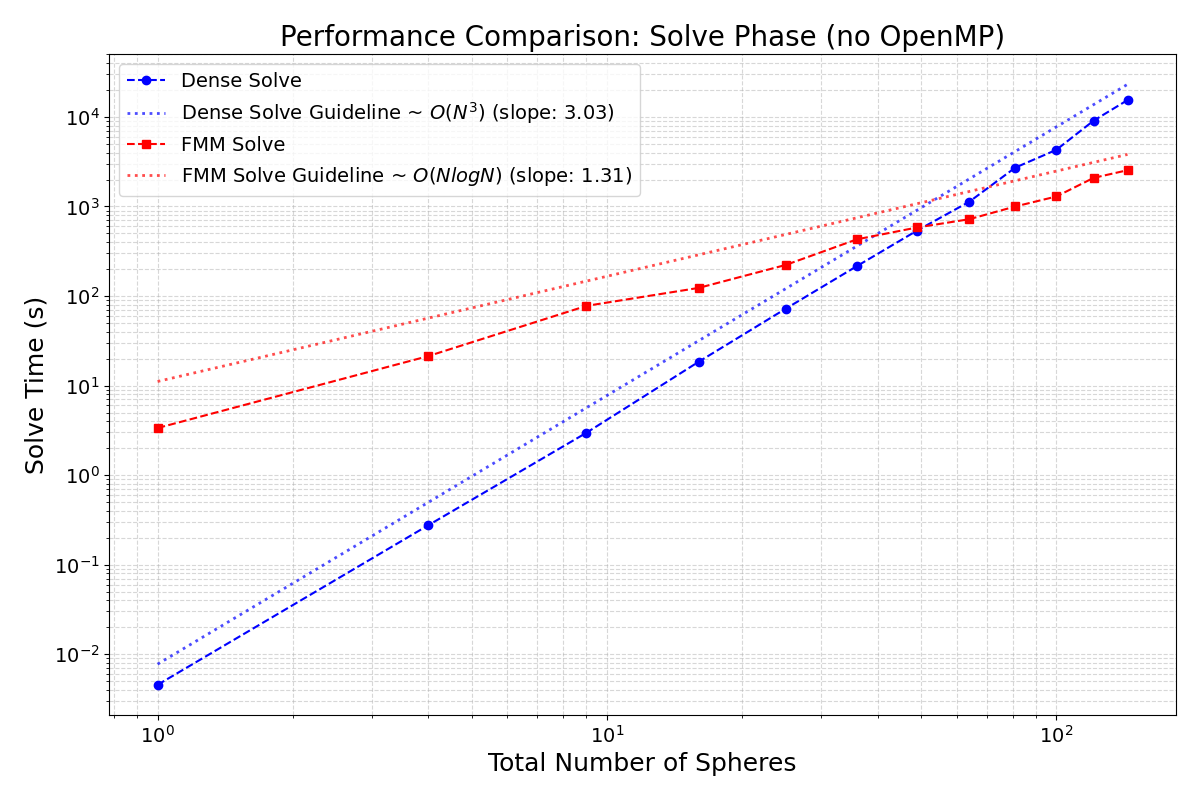
\includegraphics[width=0.8\textwidth]{figures/Timing_Compare_Plots/noOpenMP/timings_comparison_Solve_(no_openmp).png}
    \caption[Time to solve the system without OpenMP]{Time taken to solve the system for the traditional \ac{BEM}, as compared to the time taken to solve the \ac{FMM} system. The \ac{FMM} solution time scales as $\mathcal{O}(N^{\frac{3}{2}})$ with the direct \ac{BEM} solver scaling as $\mathcal{O}(N^3)$.}
    \label{fig:solve_time_comparison-no_openmp}
    
\end{figure}

\begin{figure}[htpb]
    \centering
    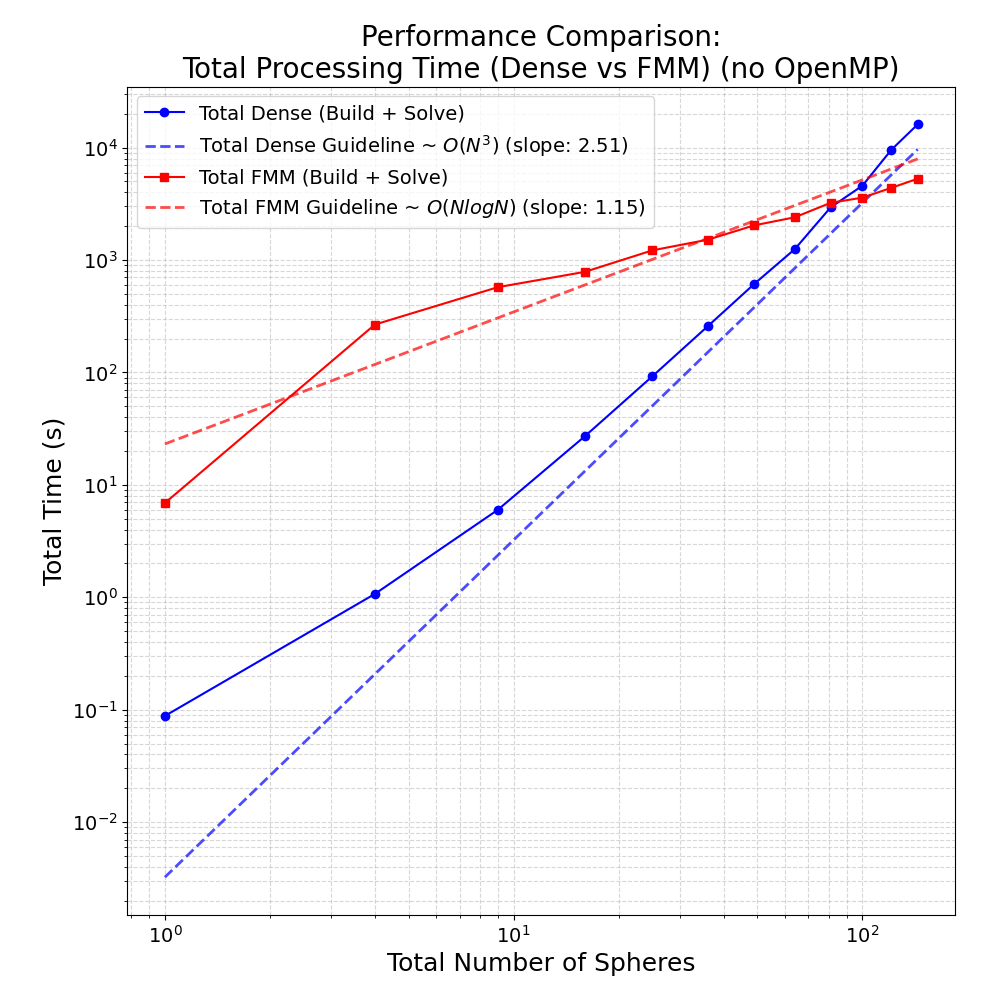
\includegraphics[width=0.8\textwidth]{figures/Timing_Compare_Plots/noOpenMP/timings_comparison_totals_(no_openmp).png}
    \caption[Total time taken without OpenMP]{Total time taken by the traditional \ac{BEM}, as compared to the time taken by the \ac{FMM}. The \ac{FMM} time complexity remains the same $\mathcal{O}(N\log N)$ in the single-threaded case, just with higher absolute times. The \ac{BEM} complexity remains $\mathcal{O}(N^3)$.}
    \label{fig:total_time_comparison-no_openmp}
    
\end{figure}